
\section{Chiusura transitiva e riflessiva}\label{chiusura-transitiva-e-riflessiva}

La chiusura riflessiva e transitiva di un grafo \emph{G = (V,E)} è il
grafo \emph{G* = (V,E*)} che si ottiene da \emph{G} aggiungendo tutti
gli archi \emph{uv} tali che in \emph{G} ci sia un cammino da \emph{u} a
\emph{v}.

Ovvero se nel grafo originale c'è un arco \emph{uv}, la chiusura
transitiva contiene gli archi che collegano \emph{u} a tutti i nodi che
possono essere raggiunti da \emph{v} e gli archi che collegano i nodi
entranti in \emph{u} a \emph{v}.

\begin{figure}[htbp]
\centering
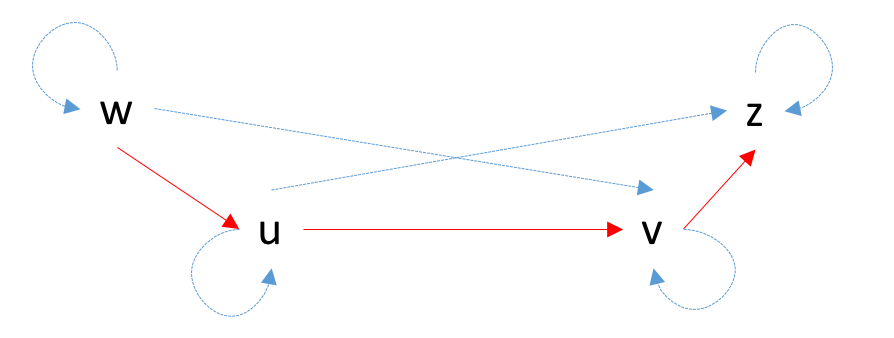
\includegraphics[width=.5\textwidth]{./notes/immagini/l3-rifle-trans.png}
\caption{Archi aggiunti nel grafo riflessivo e transitivo (in azzurro
tratteggiato), in rosso gli archi del grafo originale.}
\end{figure}

L'algoritmo naive riesce a trovare una soluzione in \emph{O(n\^{}3)}

\begin{breakablealgorithm}
	\caption{CRM/CT: Chiusura di un grafo}
	\begin{algorithmic}[1]
		\Function{CRM}{$M, M*, s$}
			\For{$u = 1 \: to \: n$}
				\For{$v = 1 \: to \: n$}
					\State $M*[u,v] \gets 0$
				\EndFor
			\EndFor
			\For{$u = 1 \: to \: n$} \Comment{Chiusura riflessiva, aggiunge i cappi}
				\State $M*[u,u] \gets 1$
			\EndFor
			\For{$u = 1 \: to \: n$}
				\For{$v = 1 \: to \: n$}
				\If {$ M[u,v] = 1 \: \text{and} \: M*[u,v] = 0 $}
					\State // Aggiungi tutti gli archi \textit{wz} con \textit{z}
					\State // raggiungibile da \textit{w} con un cammino passante per \textit{uv}
					\State \textsc{CT}$(M*,u,v,n)$
				\EndIf
				\EndFor
			\EndFor
		\EndFunction
		\Statex
		\Function{CT}{$M*,u,v,n$}
			\State $M*[u,v] \gets 1$
			\For{$z = 1 \: to \: n$}
				\If {$ M*[v,z] = 1 \: \text{and} \: M*[u,z] = 0 $}
					\State \textsc{CT}$(M*, u, z, n)$
				\EndIf
			\EndFor
			\For{$w = 1 \: to \: n$}
				\If {$ M*[w,u] = 1 \: \text{and} \: M*[w,v] = 0 $}
					\State \textsc{CT}$(M*, w, z, n)$
				\EndIf
			\EndFor
		\EndFunction
	\end{algorithmic}
\end{breakablealgorithm}

Per \textsc{CRM} l'inizializzazione della matrice \texttt{M*} ha
complessità $O(n+n^2)$, mentre l'ultimo
\texttt{for} ha complessità $O(n^2)$ (senza considerare la complessità
di \textsc{CT}. \textsc{CT} ha complessità $O(n \cdot m* )$, \emph{n}
deriva dal ciclo \texttt{for} e \emph{m*} deriva dal numero di chiamate
ricorsive che sono limitate dal numero di archi nel grafo riflessivo,
ovvero \emph{m*}.

La complessità totale è quindi $O(n^2 + n \cdot m*)$

\section{Visita in ampiezza}\label{visita-in-ampiezza}

Dato un grafo \emph{G=(V,E)} e fissato un vertice del grafo \emph{s}, la
visita in ampiezza partendo dalla \textbf{sorgente} \emph{s} visita
sistematicamente il grafo per scoprire tutti i vertici che sono
raggiungibili da \emph{s}.

In questo modo è possibile misurare la \textbf{distanza} dei vertici
dalla sorgente e costruire l'\textbf{albero della visita in ampiezza}, i
cui rami sono i cammini di lunghezza minima che partono dalla sorgente e
raggiunto tutti i vertici del grafo che possono essere raggiunti.

Tutti i cammini che compaiono nell'albero della visita in ampiezza sono
tutti \textbf{cammini minimi}.

La vista in ampiezza parte quindi da \emph{s} e visita tutti i vertici a
distanza 1, per poi passare a quelli a distanza 2 e così via, ovvero la
frontiera dell'albero viene espansa in ampiezza.

Durante l'esplorazione un nodo può essere colorato in tre modi:

\begin{itemize}
\item
  \textbf{bianco}: vertice del grafo non ancora raggiunto
\item
  \textbf{grigio}: vertice raggiunto e che si trova sulla frontiera,
  ovvero non sono stati ancora raggiunti tutti i suoi figli
\item
  \textbf{nero}: vertice raggiunto e che non si trova più nella
  frontiera.
\end{itemize}

Ad alto livello, l'algoritmo parte dal vertice \emph{s} utilizzandolo
come radice dell'albero. Quando viene scoperto un vertice bianco
\emph{v} a causa di un arco \emph{uv} che lo connette al vertice \emph{u}
scoperto precedentemente (all'inizio \emph{u=s}), questo viene aggiunto
all'albero e collegato al nodo \emph{u}, che diventa il \textbf{padre}
di \emph{v}.

L'implementazione dell'algoritmo utilizza una coda FIFO \textbf{Q} che
mantiene in memoria la frontiera.

\begin{figure}[htbp]
\centering
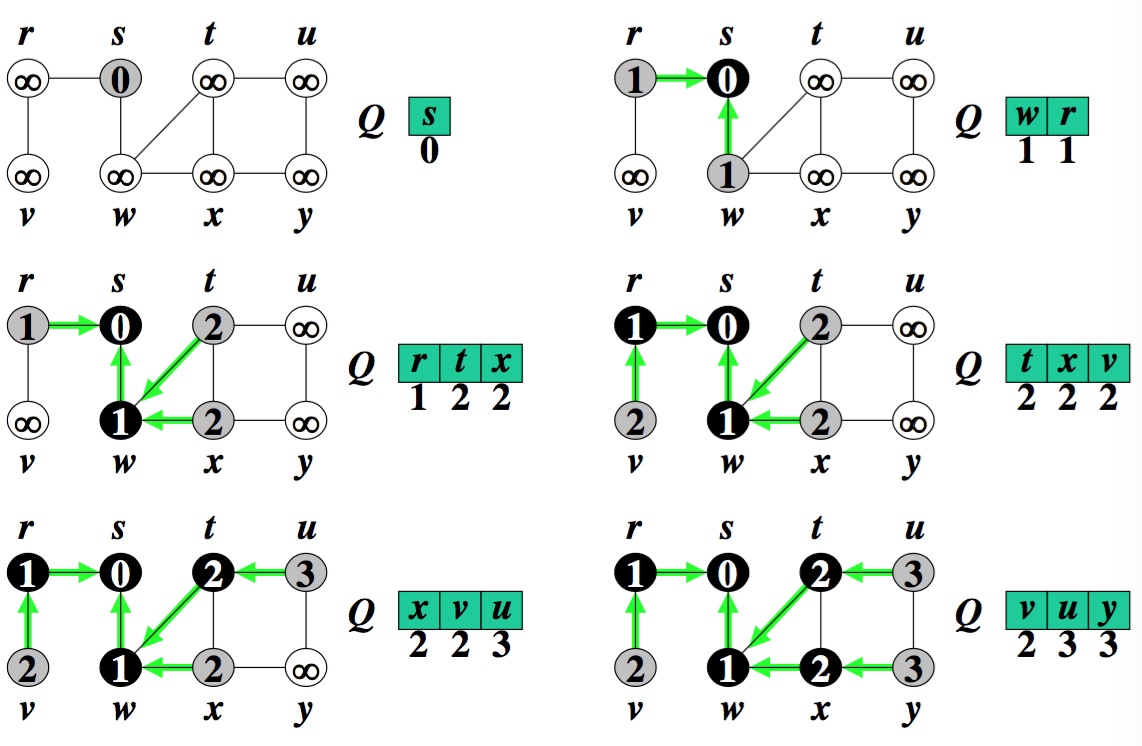
\includegraphics[width=.8\textwidth]{./notes/immagini/l3-ampi.png}
\caption{Esplorazione in ampiezza}
\end{figure}

\begin{breakablealgorithm}
	\caption{BFS: Esplorazione in ampiezza di un grafico}
	\begin{algorithmic}[1]
		\Function{BFS}{$ G,s $}
			\For{$ \forall v \in G.V $}
				\State $ v.color \gets \text{bianco} $ 
				\State $ v.d \gets \infty $ \Comment{Distanza massima possibile}
				\State $ v.\pi \gets nil $\Comment{Padre del nodo}
			\EndFor
			\State $ s.color \gets \text{grigio} $
			\State $ s.d \gets 0 $
			\State \textsc{Push}$ (Q,s)$
			\While{not \textsc{Empty}\textit{(Q)}}
				\State $ u \gets $ \textsc{Pop}$ (Q) $
				\For{$ \forall v \in Adj[u] $}
					\If{$ v.color = $ bianco}
						\State $ v.color \gets \text{grigio} $ 
						\State $ v.d \gets u.d + 1 $
						\State $ v.\pi \gets u $
						\State \textsc{Push}$ (Q,v) $
					\EndIf
				\EndFor
				\State $ u.color = $ nero
			\EndWhile
		\EndFunction
	\end{algorithmic}
\end{breakablealgorithm}

\subsection{Complessità}\label{complessituxe0}

Il ciclo \texttt{for} di inizializzazione ha complessità \emph{O(n)}.

Il ciclo \texttt{while} viene ripetuto al massimo \emph{n} volte e il
\texttt{for} interno percorre la lista delle adiacenze di tutti i nodi,
al massimo una volta sola, quindi le iterazioni totali dei cicli
\texttt{for} sono \emph{m}. In tutto il ciclo
\texttt{while} ha complessità \emph{O(n+m)}, la quale domina la
complessità dell'inizializzazione.

La complessità dell'algoritmo è anche ottima, non è possibile ottenere
una visita completa del grafo effettuando meno di \emph{O(n+m)}
operazioni.

Da notare che $O(n*m)$ sarebbe sbagliata come complessità, perché $m$
tiene in considerazione il fatto che il ciclo \texttt{for} viene
ripetuto $n$ volte.

\subsection{Correttezza}\label{correttezza}

Indichiamo con $\delta(u,v)$ la distanza tra il vertice \emph{v} e
\emph{u}, ovvero la lunghezza del cammino minimo che li congiunge. Per
convezione, se i due vertici non sono raggiungibili, la distanza è
infinita.

La distanza così definita ha la proprietà (\textbf{proprietà delle distanze}) 

$$\delta(x,v) \leq \delta(x,u) + 1 \text{ per ogni } x \in V \text{ e } uv \in E$$
 
Questo perché aggiungendo l'arco \emph{uv} al cammino $ x \rightarrow u$, si ottiene un cammino di
lunghezza $\delta(x,u) + 1$, pertanto, per definizione $\delta(x,v)$ è
minore o uguale della lunghezza del nuovo cammino.

Un'altra proprietà è quella del \textbf{limite superiore}, ovvero per
ogni vertice \emph{u} e per tutta l'esecuzione di \textbf{BFS} vale la
disuguaglianza $u.d \geq \delta(s,u)$.

Questo è trivialmente vero per \emph{s.d} e per \emph{u.d} quando \emph{u} non è raggiungibile da \emph{s} (per costruzione).

L'unica istruzione dell'algoritmo che modifica la distanza è
$v.d\ =\ u.d\ + 1$, che viene eseguita solo se esiste l'arco
\emph{uv}. Supponendo induttivamente che la proprietà sia vera prima di
eseguire l'assegnamento, si ha che:

\begin{align*}
v.d &= u.d + 1 &\\
     &\geq \delta(s,u) + 1 & \text{// per l'ipotesi induttiva }\\
     &\geq \delta(s,v)   & \text{// per la proprietà delle distanze}
\end{align*}

Un'altra proprietà utile alla dimostrazione di correttezza è che, se la
coda \emph{Q} non è vuota, allora è ordinata per distanza crescente.

Formalmente

$$
v_1, v_2, \ldots, v_r \in Q \: | \:  v_i.d \leq v_{i+1}.d + 1 \: \forall i \: \text{ e } \: v_r \leq v_1.d +1
$$

Questa proprietà è vera per la coda con un solo elemento, la quale è
sempre ordinata.

Induttivamente, le operazioni che modificano la coda sono i push e i
pop.

Quando viene eseguito un pop, viene tolto il primo elemento e la
proprietà rimane vera perché $v_r.d \leq v_1.d + 1 \leq v_2.d + 1$.

Nel caso di un push con la coda che contiene già degli elementi
ordinati, questa operazione viene eseguita dopo aver tolto dalla coda il
vertice \emph{u} e viene aggiunto il nodo \emph{v} con \emph{v.d = u.d +
1}.

Dopo aver rimosso \emph{u}, il primo elemento dello coda ha  $v_1.d \leq u.d + 1$ e l'ultimo elemento $v_r$ ha distanza
$v_r.d \leq u.d +1$. Dal momento che viene aggiunto in
coda \emph{v} con \emph{v.d = u.d + 1}, si ha che $v_r.d \leq v.d$, pertanto la proprietà rimane soddisfatta.
